\begin{figure}[h]
    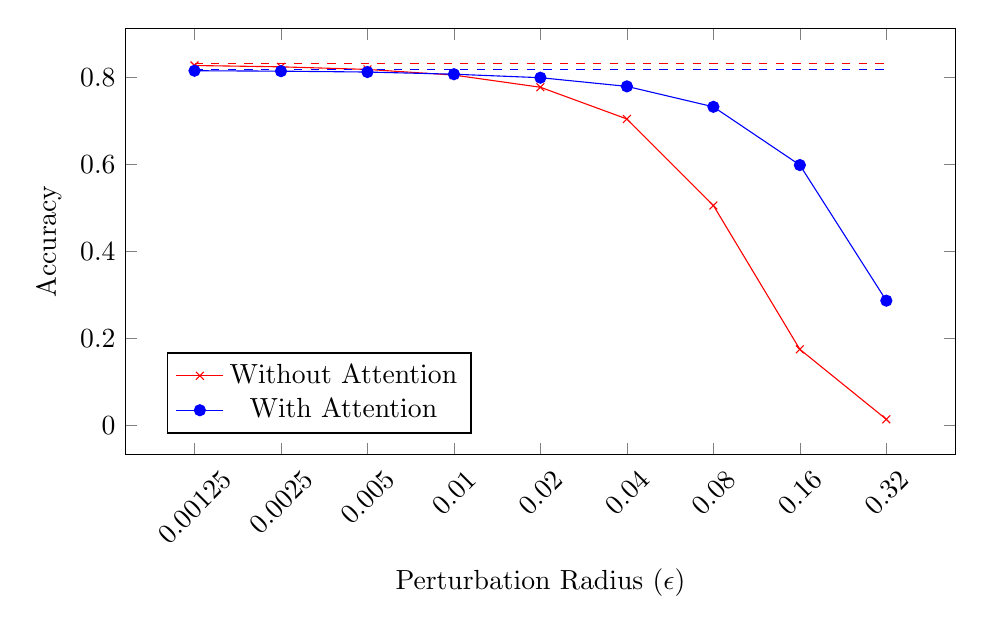
\begin{tikzpicture}
      \begin{axis}[xtick={0, 0.00125, 0.0025, 0.005, 0.01, 0.02, 0.04, 0.08, 0.16, 0.32}, x tick label style={rotate=45, log ticks with fixed point},xmode=log, log basis x=2, xlabel=Perturbation Radius ($\epsilon$), ylabel=Accuracy, width=\linewidth, height=7cm,legend style={at={(0.05,0.05)},anchor=south west}]
          
      \addplot[color=red,mark=x] coordinates {
        (0, 0.832)
        (0.00125, 0.828)
        (0.0025, 0.825)
        (0.005, 0.819)
        (0.01, 0.806)
        (0.02, 0.778)
        (0.04, 0.705)
        (0.08, 0.506)
        (0.16, 0.175)
        (0.32, 0.014)
      };
      
      \addplot[color=blue,mark=*] coordinates {
        (0, 0.818)
        (0.00125, 0.816)
        (0.0025, 0.815)
        (0.005, 0.813)
        (0.01, 0.808)
        (0.02, 0.8)
        (0.04, 0.780)
        (0.08, 0.733)
        (0.16, 0.599)
        (0.32, 0.287)
      };

      \addplot[color=red, domain=0.00125:0.32, dashed]{0.832};
      \addplot[color=blue, domain=0.00125:0.32, dashed]{0.818};
      
      \legend{Without Attention,With Attention}
      \end{axis}
      \end{tikzpicture}
    \caption{Clean- and robust-accuracy of ResNet-50 models for diabetic retinopathy detection. Dashed lines represent clean-accuracy.}
    \label{DRResNet50Robustness}
  \end{figure}